\begin{frame}[fragile]{Tracking: Snapshots, Not Differences}
  \begin{columns}
    \begin{column}{0.6\textwidth}
      \begin{figure}
        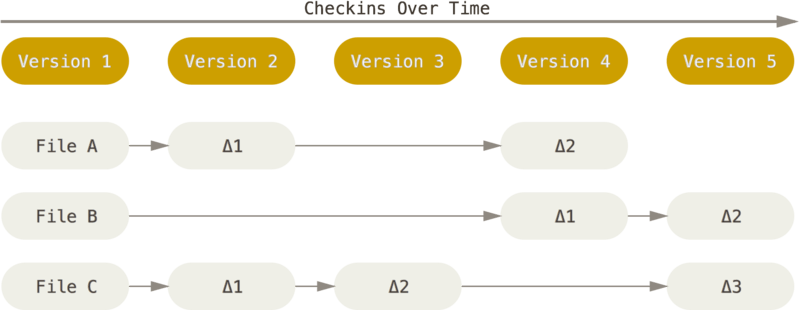
\includegraphics[width=\textwidth]{tracking/deltas}
        \caption{Storing data as differences}
      \end{figure}
      \begin{figure}
        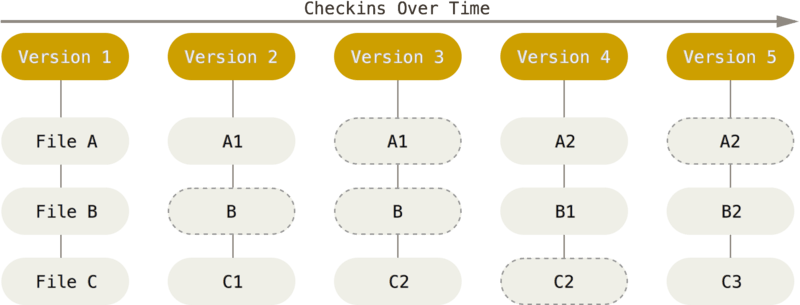
\includegraphics[width=\textwidth]{tracking/snapshots}
        \caption{Storing data as snapshots}
      \end{figure}
    \end{column}
    \begin{column}{0.4\textwidth}
      With deltas
      \begin{itemize}
          \footnotesize
          \item Most other VCSs store information as a list of file-based changes (deltas)
          \item Space efficient
      \end{itemize}
      With snapshots
      \begin{itemize}
          \footnotesize
          \item Fetches the history instantly
          \item Calculates the differences on the fly
          \item Imitates a Unix-style file system
          \item Improves branching
      \end{itemize}
    \end{column}
  \end{columns}
\end{frame}
